% Itemizing
\begin{enumerate}[label=(\alph*)]

% A basic table from Section 1.1.
\begin{table}[ht!]
\begin{centering}
\begin{tabular}{l*{5}{r}}
\toprule
{\bf Circumference:} $c$ (feet) & 1.7 & 2.5 & 5.5 & 8.2 & 13.7\tabularnewline
\midrule
{\bf Height:} $h$ (feet) & 24.5 & 31.0 & 45.2 & 54.6 & 92.1\tabularnewline
\bottomrule
\end{tabular}
\caption{Height of a tree as a function of its circumference.}
\label{tab:1-tree}
\end{centering}
\end{table}

% A table with fractions. Table 2.1.
\begin{table}[ht!]
\begin{centering}
\begin{tabular}{lll}
\toprule
$\Delta t$ (seconds) & $\Delta h = h(1+\Delta t)-h(1)$ (feet) & $\dfrac{\Delta h}{\Delta t}$ (ft/s) \\
\midrule
1       & $h(2) - h(1) = 36-84 = -48$                   & $\dfrac{-48\mathstrut}{1\mathstrut} = -48$ \\
0.5     & $h(1.5) - h(1) = 64-84 = -20$                 & $\dfrac{-20\mathstrut}{0.5\mathstrut} = -40$ \\
0.1     & $h(1.1) - h(1) = 80.64-84 = -3.36$            & $\dfrac{-3.36\mathstrut}{0.1\mathstrut} = -33.6$ \\
0.01    & $h(1.01) - h(1) = 83.6784-84 = -0.3216$       & $\dfrac{-0.3216\mathstrut}{0.01\mathstrut} = -32.16$ \\
0.001   & $h(1.001) - h(1) = 83.967984-84 = -0.032016$  & $\dfrac{-0.032016\mathstrut}{0.001\mathstrut} = -32.016$ \\
\bottomrule
\end{tabular}
\caption{Average velocities approaching the instantaneous velocity at $t=1$ seconds.}
\label{tab:2-2-tomato-velocity}
\end{centering}
\end{table}

% A centered figure from Section 2.2.
\begin{figure}[!ht]
  \centering
    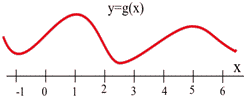
\includegraphics[width=0.4\textwidth]{img/chap2/image006.png}
    \caption{$y=g(x)$}
    \label{fig:2-2-gx}
\end{figure}

% Wrapped figure in Chapter 0 (not in an itemized environment.

\begin{wrapfigure}{R}{0.25\textwidth}
  \vspace{-20pt}
  \centering
    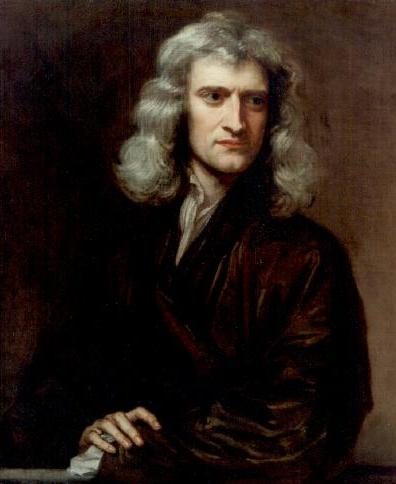
\includegraphics[width=0.24\textwidth]{img/chap0/IsaacNewton.jpg}
%\vspace{-20pt}  
\caption{Isaac Newton in 1689}
\label{fig:0-newton}
\vspace{-10pt}
\end{wrapfigure}

% Wrapped figure for an itemized environment.
% In Exercises 1.1.6
\begin{minipage}{\linewidth}
\begin{wrapfigure}{r}{0.4\textwidth}
    \centering
    \vspace{-12pt}
    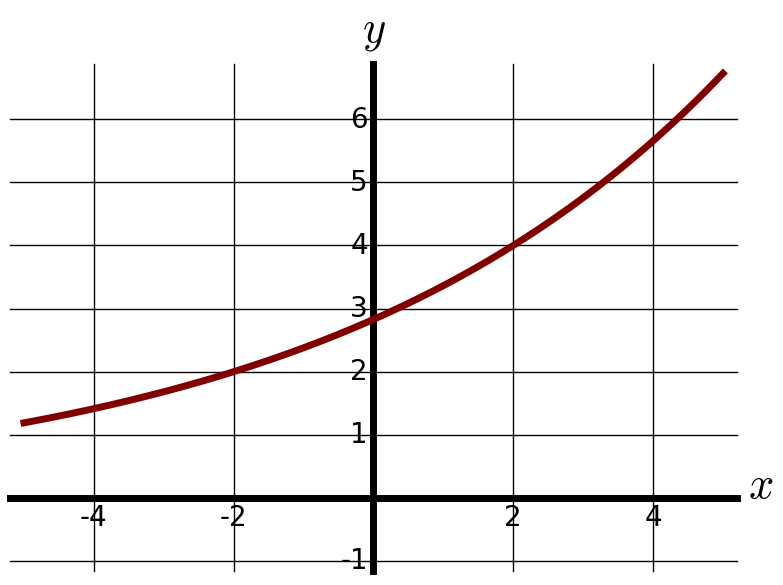
\includegraphics[width=0.4\textwidth]{img/chap1/sec1-2/prob7.png}
\end{wrapfigure}

\item Let $g(x)$ be the function graphed on the right.
    \begin{enumerate}
        \item Evaluate $g(2)$.
        \item Solve $g(x) = 2$ for $x$.
    \end{enumerate}
\end{minipage}

% Sample Spreadsheet
\begin{table}[!ht]
  \centering
  \textsf{
  \begin{tabular}{|a*{10}{|c}|}
    \hline
    \rowcolor{shGray} & A & B & C & D & E & F & G & H & I & J\\
    \hline
      1 & \textbf{Chirps} & 44 & 35 & 20.4 & 33 & 31 & 35 & 18.5 & 37 & 26 \\
    \hline
      2 & \textbf{Temp. ($^{\circ}$F)} & 80.5 & 70.5 & 57 & 66 & 68 & 72 & 52 & 73.5 & 53\\
    \hline
  \end{tabular}}
  \caption{}
  \label{sh:crickets}
\end{table}

% Sample Graph with points.
% Example 0.1.1

\begin{figure}[ht!]
\centering
\begin{tikzpicture}[scale=0.09]
    % grid
    \draw[step=10, very thin, gray] (0, 0) grid (40, 60);

    % axes
    \draw[->] (-2,0) -- coordinate (x axis mid) (42,0) node[right] {$x$};
    \draw[->] (0,-2) -- coordinate (y axis mid) (0,63) node[above] {$y$};

    % ticks
    \foreach \x in {10, 20, ..., 40}
     		\draw (\x,1pt) -- (\x,-3pt)
			node[anchor=north] {\x};
    	\foreach \y in {100, 200, ..., 600}
     		\draw (1pt,\y/10) -- (-3pt,\y/10) 
     			node[anchor=east] {\y}; 

    % labels
    \node[below = 15] at (x axis mid) {Hours worked};
	\node[rotate=90, above = 25] at (y axis mid) {Pay (U.S.\ Dollars)};

    % plot 
    \draw[->, very thick, color=aldRed] (0, 0) -- (42, 63);
    
    % points
    \filldraw (0, 0) circle [radius=20pt]; %node[left, fill=white] {$(0,0)$};
    \filldraw (20, 30) circle [radius=20pt]; %node[below right, fill=white] {$(20,300)$};
    % legend

\end{tikzpicture}
\caption{Pay as a function of time worked.}
\label{fig:0-rate}
\end{figure}

% Sample graph with shading
% Example 0.2.1

\begin{figure}[ht!]
\centering
\begin{tikzpicture}[scale=1]
    % grid
    \draw[step=1, very thin, gray] (0, 0) grid (12, 3);

    % axes
    \draw[->] (-0.2,0) -- coordinate (x axis mid) (12.5,0) node[right] {$t$};
    \draw[->] (0,-0.2) -- coordinate (y axis mid) (0,3.5) node[above] {$y$};

    % ticks
    \foreach \x in {1, 2, ..., 12}
     		\draw (\x,1pt) -- (\x,-3pt)
			node[anchor=north] {\x};
    	\foreach \y in {1, 2, 3}
     		\draw (1pt,\y) -- (-3pt,\y) 
     			node[anchor=east] {\y}; 

    % labels
    \node[below= 15] at (x axis mid) {Time (hours)};
	\node[rotate=90, above= 25] at (y axis mid) {Snowfall rate (in/hr)};

    % plot
    \fill[color=aldBlue!30, opacity=0.5] (0, 0) -- (4, 1) -- (6,2) --(8, 2) -- (12, 0);
	\draw[very thick, color=aldRed] (0, 0) -- (4, 1) -- (6,2) --(8, 2) -- (12, 0); 
    
    % legend
    \node [fill=white] at (7, 2.5) {$y=r(t)$};

 \end{tikzpicture}
\caption{Snowfall rate during a snowstorm.}
\label{fig:0-snow}
\end{figure}

% Plot a collection of points, with built-in x- and y-scaling.
% Example 2.2.4.
\begin{tikzpicture}[scale=2]
    \def\xmin{0}
    \def\xmax{2.5}
    \def\xscale{1}

    \def\ymin{0}
    \def\ymax{100}
    \def\yscale{40}

    % grid
    \draw[step=0.5, very thin, gray] (\xmin/\xscale, \ymin\yscale) grid (\xmax/\xscale, \ymax/\yscale);

    % axes
    \draw[->] (-0.2,0) -- coordinate (x axis mid) (2.7, 0) node[right] {$t$};
    \draw[->] (0,-0.2) -- coordinate (y axis mid) (0, 2.7) node[above] {$y$};

    % ticks
    \foreach \x in {0.5, 1, ..., 2.5}
     		\draw (\x,1pt) -- (\x,-3pt)
			node[anchor=north] {\x};
    	\foreach \y in {20, 40, ..., 100}
     		\draw (1pt,\y/\yscale) -- (-3pt,\y/\yscale) 
     			node[anchor=east] {\y}; 

    % labels
    \node[below = 15] at (x axis mid) {Time (seconds)};
	\node[rotate=90, above = 25] at (y axis mid) {Height (feet)};

    % plot 
    
    % points
    \foreach \pt in {(0, 100/\yscale), (0.5, 96/\yscale), (1, 84/\yscale), (1.5, 64/\yscale), (2, 36/\yscale), (2.5,0/\yscale)}
        \filldraw[color=aldRed] \pt circle [radius=2pt]; 
    % legend

\end{tikzpicture}

% Sample plot with a function.
% For Example 2.2.1

\begin{figure}[ht!]
\centering
\begin{tikzpicture}[scale=1]
    % grid
    \draw[step=1, very thin, gray] (0, 0) grid (10, 6);

    % axes
    \draw[->] (-0.2,0) -- coordinate (x axis mid) (10.5,0) node[right] {$t$};
    \draw[->] (0,-0.2) -- coordinate (y axis mid) (0, 6.5) node[above] {$y$};

    % ticks
    \foreach \x in {1, 2, ..., 10}
     		\draw (\x,1pt) -- (\x,-3pt)
			node[anchor=north] {\x};
    	\foreach \y in {1, 2, ..., 6}
     		\draw (1pt,\y) -- (-3pt,\y) 
     			node[anchor=east] {\y}; 

    % labels
    \node[below = 15] at (x axis mid) {Time (hours)};
	\node[rotate=90, above = 25] at (y axis mid) {Bacteria population (millions)};

    % plot 
    \draw[smooth, samples=1000, domain=0:10.2, very thick, color=aldRed] plot(\x,{(6*\x+2)*exp(-\x/2)});    

    % points
   
    % legend

\end{tikzpicture}
\caption{Population of a bacteria culture $t$ hours after an antibiotic is added.}
\label{fig:2-2-bacteria}
\end{figure}

% Sample for a grid
\begin{center}
\begin{tikzpicture}
  \begin{axis}[
    xmin = -2, xmax = 202,
    ymin = -2, ymax = 152,
    xtick distance = 50,
    ytick distance = 50,
    grid = both,
    major grid style = {gridGray},
    width = 0.6\textwidth,
    xlabel = {Distance traveled (miles) ($m$)},
    ylabel = {Total Cost (\$)},
    legend cell align = {left},
    legend pos = north west
    %height = 0.5\textwidth,
    ]
    \filldraw (100, 79) circle (2pt) node[below right] {$(100, 79)$};
    \addplot[domain = 0:202, samples = 2, smooth, thick, aldRed] {20 + 0.59*x};
    \addplot[domain = 0:202, samples = 2, smooth, thick, aldBlue] {16 + 0.63*x};
    \legend{ $Y(m) = 20 + 0.59 m$,
             $B(m) = 16 + 0.63 m$}

\end{axis}
\end{tikzpicture}
\end{center}

% Sample for a time series taken from a data file.
% Example 2.1.1
\begin{wrapfigure}{R}{0.5\textwidth}
  \vspace{-20pt}
\centering
\begin{tikzpicture}[scale=1]
    \begin{axis}[
        date coordinates in=x,
        date ZERO=2019-12-31,
        ytick distance = 5,
        grid = both,
        major grid style = {gridGray},
        xticklabel = {\year-\month},
        ylabel = {Price ($\$10,000$)},
    ]
    \addplot[very thick, aldRed, mark=*] table[x=Date, y=Price] {datasets/bitcoin2020.dat};
    \end{axis}
\end{tikzpicture}
\caption{Price of Bitcoin in 2020, in Thousands of Dollars. Source: Coindesk; https://www.coindesk.com/price/bitcoin}
\label{fig:2-1-bitcoin2020}
\end{wrapfigure}


\begin{center}
\begin{tikzpicture}
  % Grid
  \draw[help lines] (-0.2, -0.2) grid (6.2, 5.2); % Grid
  \draw[->] (-0.2, 0) -- (6.2, 0) node[right] {$x$}; % x-axis
  \draw[->] (0, -0.2) -- (0, 5.2) node[above] {$y$}; % y-axis
  % Axis labels
  \foreach \x/\xtext in {1, 2, 3, 4, 5, 6}
     \draw (\x cm,1pt) -- (\x cm,-1pt) node[anchor=north,fill=white] {$\xtext$};
   \foreach \y/\ytext in {1, 2, 3, 4, 5}
     \draw (1pt,\y cm) -- (-1pt,\y cm) node[anchor=east,fill=white] {$\ytext$};
   \node[below left](origin) at (0, 0){0};
  % Points
  \filldraw (0, 5) circle [radius=2pt];
  \filldraw (3, 3) circle [radius=2pt];
  \filldraw (6, 1) circle [radius=2pt];

  %Line
  \draw[color=aldRed, thick, domain=-0.2:6.2] plot(\x, 5 - 2*\x/3) node[right] {$f(x) = 5 - \frac{2}{3} x$};
\end{tikzpicture}
\end{center}
